

\chapter{Sprint 1}
\label{Sprint0}
\lhead{Chapter 7. \emph{Sprint 1}}

\section{Goal(s)}
This sprint's goal was the completition of an initial prototype of the system whose functionality
had to be demonstrated to the customer using an Android application. This corresponded to project milestone M1.

\section{Planning}
In order the achive the goal for this sprint we planned to begin coding the functionality required to demonstrate
the system as a whole. This led to an initial design and implementation of every part of the system including:
a) the frontend b) the backend and database c) the Android application.
%We had planned some work on the report as well but that got moved to another iteration due to..

\section{Duration}
The duration of the sprint was the following:
\begin{itemize}
\item Start: September, 9th
\item End: September, 22nd
\end{itemize}

\begin{figure}[H]
\centering
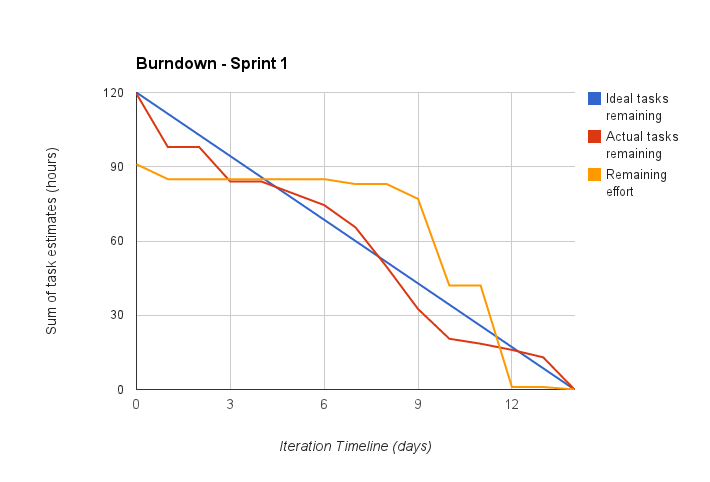
\includegraphics[scale=0.60]{../Figures/burndownSprint1.png}
\caption{Burndown chart Sprint 0}
\label{figure:burndownsprint0}
\end{figure}

\section{Backlog}

See below the ordered sprint backlog.
\begin{itemize}
	\item \textbf{M1 First system prototype}
	\item \textbf{Project management}\newline
	This included:
	\begin{itemize}
		\item \textbf{Weekly startup meeting}: 
		\item \textbf{Meeting notes}:
			taking notes during meetings, reviewing of the notes.
		\item \textbf{Status reports}:
			for both week 37 and 38
		\item \textbf{Risk analysis}:
			updated on a weekly basis, so twice per sprint.
			The risk analisys was submitted to the supervisor and the customer.
		\item \textbf{Planning for the next iteration}:
			the project manager prepared a plan for the next iteration
			which would be illustrated and agreed upon on next iteration's startup meeting.
	\end{itemize}
	\item \textbf{Weekly meetings}
		includes meetings with both the customer and the supervisor.
		The meeting with the customer was held on Skype.
	\item \textbf{Additional pre-studies}
		Continued studies on relevant technlogies such as:
	\begin{itemize}
		\item \textbf{Studies on HealthVault}
		\item \textbf{Studies on Apache Camel}
		\item \textbf{Studies on JS chart libraries}
	\end{itemize}
	\item \textbf{System development}
		Initial design and implementation. For this sprint, this accounted for:
	\begin{itemize}
		\item \textbf{Backend development}:
			Initial Spring controllers for API endpoints and database (DAO) development.
		\item \textbf{Frontend development}:
			Coding of the frontend using JS to implement charts.
		\item \textbf{Deployment}:
			Deployment of both backend and frontend.
	\end{itemize}
	\item \textbf{Heart rate application}:
		Basic implementation of the Heart rate application. The application should be able to acquire
		the user's heart reate and send perform a REST API call to store the data on the backend.
	\item \textbf{Database development}:
		We chose a suitable database to use for implementing persistency on the backend.
		We opted for MySQL due to the familiarity we had with it. We then deployed it on the server machine
		and added a table so that we could test the functionality of the backend.
	\item \textbf{Testing}:
		Perform unit and integration testing for the heart rate application and the backend.
\end{itemize}


%% i actually dont think having a table for this is a good idea. tables can't have much information
%% also it would require a lot of tweaking to get the estimated/actual times to look reasonable.
%% maybe a textual description would be better so we can omit some details in favor of others.
\iffalse
\begin{table}
\begin{tabular}{ | l | l | l | l | }
 \hline
  Story ID & Description & Size & Assignee \\
  \hline\noalign{\smallskip}\noalign{\smallskip}\hline
  33 & Project Management			& 8	& Emanuele  \\
  12 & M1 First System prototype	& 0 & All		\\
  45 & Weekly meetings (week 37)	& 6 & All		\\
  42 & Additional pre-studies		& 5 & Emanuele	\\
  \hline
\end{tabular}
\caption{}
\label{}
\end{table}
\fi

\section{Testing}

\section{Results and feedback}
We presented a prototype of the product to the customer and he seemed to be very pleased with the results.
He stated that the results were above his expectations.
We talked about some features that he'd would like to see implemented in the product
and we agreed to prioritise HealthVault interoperability.

\section{Evaluation}
We manage to achived what we had planned for this sprint.
We received positive feedback and ultimately pinned down some refined requirements of the product.